\chapter{Ekosystem Dockera}

Pojęcie Docker jest powiązane z~kilkoma znaczeniami. Po pierwsze jest to specyfikacja obrazów kontenera i~środowiska wykonawczego, w~tym plików \textit{Dockerfile}, umożliwiających powtarzalny proces budowania (rys.~\ref{fig:ecosystem}a). Ponadto, jest to także oprogramowanie, które implementuje tę specyfikację (demon Docker, o~nazwie Docker Engine, rys.~\ref{fig:ecosystem}b), centralny rejestr, w~którym programiści mogą przechowywać i~udostępniać swoje obrazy (Docker Hub, rys.~\ref{fig:ecosystem}c) oraz inne nieoficjalne rejestry (rys.~\ref{fig:ecosystem}d), wraz ze znakiem towarowym (Docker Inc.). Proces rozwoju oprogramowania zakłada przetrzymywanie kodu w~zewnętrznym repozytorium (rys.~\ref{fig:ecosystem}e) oraz wykorzystanie zewnętrzenego serwisu rurociągu CI/CD (rys.~\ref{fig:ecosystem}g). Definicja rurociągu łączy zdefiniowany kod z~zewnętrznymi zależnościami (rys.~\ref{fig:ecosystem}f) i~buduje obraz Dockera, który jest publikowany we wspomnianych już rejestrach. Do zarządzania cyklem życia infrastruktury operacyjnej można wykorzystać orkiestratora (rys.~\ref{fig:ecosystem}h).

Projekt Docker został napisany w~języku Go i~wydany po raz pierwszy w~marcu 2013 roku. Od tego czasu doznał gwałtownego wzrostu popularności i~został powszechnie przyjęty przez przemysł IT jako domyślne rozwiązanie kontenerowe.

\begin{figure}[p]
    \centering
    \includegraphics[width=0.9\linewidth]{images/ecosytem.png}
    \caption{Przegląd ekosystemu Docker. Strzałki pokazują ścieżkę kodu}
    \label{fig:ecosystem}
\end{figure}

\section{Specyfikacje Dockera}

\begin{figure}[ht]
    \centering
    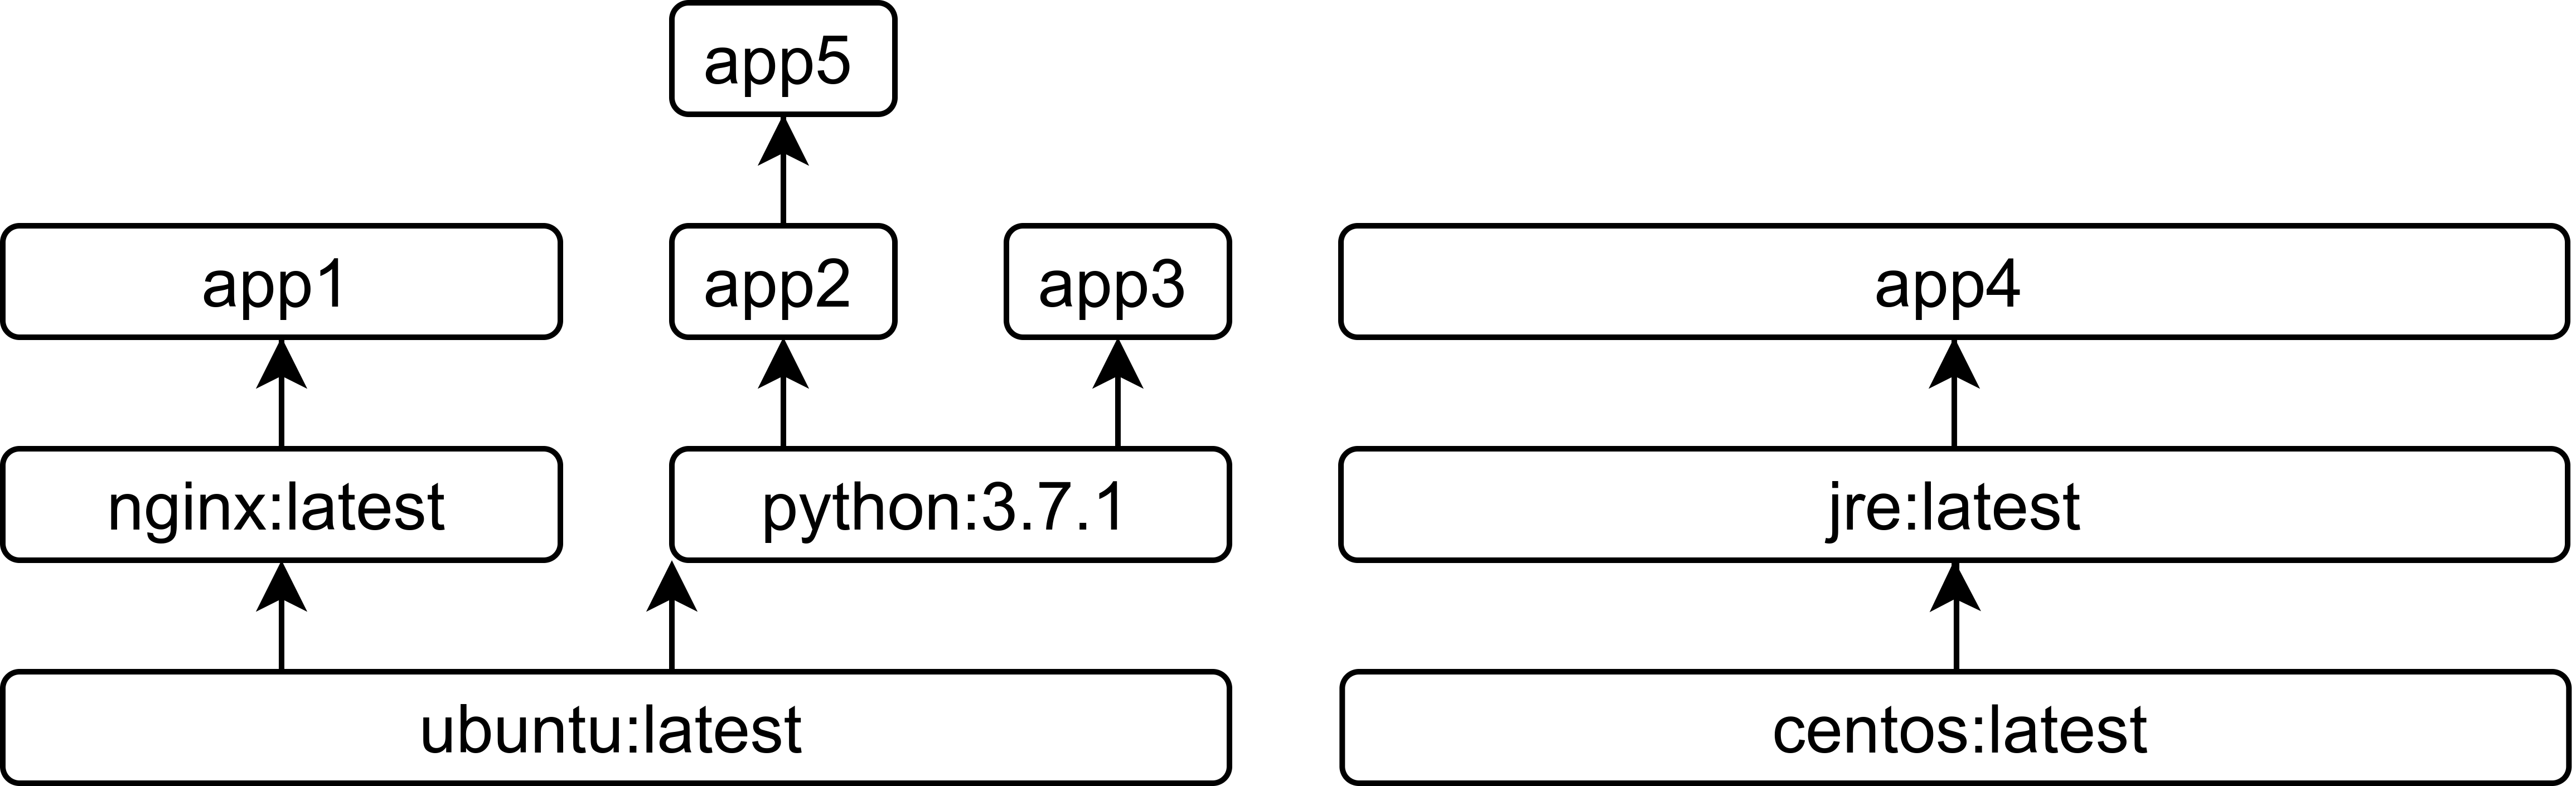
\includegraphics[width=0.9\linewidth]{images/inheritanceTree.png}
    \caption{Przykład drzew dziedziczenia obrazów}
    \label{fig:inheritanceTree}
\end{figure}

Zakres specyfikacji obejmuje obrazy kontenera i~środowisko wykonawcze. Obrazy Dockera składają się z~zestawu warstw wraz z~metadanymi w~formacie JSON. Są one przechowywane w~\textit{/var/lib/docker/$<$driver$>$/}, gdzie \textit{$<$driver$>$} oznacza używany sterownik pamięci (np.~AUFS, BTRFS, VFS, Device Mapper, OverlayFS). Każda warstwa zawiera modyfikacje wprowadzone w~systemie plików w~stosunku do poprzedniej warstwy, zaczynając od obrazu podstawowego (zazwyczaj lekkiej dystrybucji Linuxa). W~ten sposób obrazy są zorganizowane w~drzewa, a~każdy obraz ma rodzica, z~wyjątkiem obrazów podstawowych, które są korzeniami drzew (rys.~\ref{fig:inheritanceTree}). Ta struktura umożliwia wysyłanie w~obrazie tylko modyfikacji specyficznie związanych z~tym obrazem (dane właściwe aplikacji). Dlatego jeśli wiele obrazów na systemie operacyjnym gospodarza dziedziczy po tym samym obrazie podstawowym lub ma te same zależności, zostaną one pobrane tylko raz z~rejestru. Ponadto, jeśli pozwala na to lokalny sterownik pamięci (z systemem plików typu \textit{union}, tj. systemem plików tylko do odczytu i~dodatkową warstwą zapisu), będzie on przechowywany tylko raz na dysku, prowadząc do znacznych oszczędności zasobów dyskowych. Szczegółowa specyfikacja obrazów Dockera i~kontenerów znajduje się w~\cite{MobyDockerImageSpecification}.

Metadane obrazów zawierają informacje o~samym obrazie (np.~identyfikator, suma kontrolna, tagi, rejestr, autor), o~jego rodzicu (identyfikator) wraz z~opcjonalnymi parametrami środowiska wykonawczego, które posiadają wartości domyślne (np.~przekierowanie portów, konfiguracja \textit{cgroups}). Parametry te można nadpisać w~czasie uruchamiania przekazując ich wartości do komendy \textit{docker run}.

Budowanie obrazów można wykonać na dwa sposoby. Możliwe jest uruchomienie kontenera z~istniejącego obrazu (\textit{docker run}), wykonanie modyfikacji i~instalacji wewnątrz kontenera, zatrzymanie kontenera, a~następnie zapisanie stanu kontenera jako nowego obrazu (\textit{docker commit}). Proces ten jest zbliżony do klasycznej instalacji maszyny wirtualnej, ale musi być wykonywany przy każdej przebudowie obrazu (np.~w~celu aktualizacji). Z~racji, iż obraz podstawowy jest znormalizowany, sekwencja poleceń jest dokładnie taka sama. 

W celu automatyzacji powyższego procesu, pliki \textit{Dockerfile} pozwalają określić obraz podstawowy i~sekwencję poleceń, które należy wykonać w~celu zbudowania obrazu, wraz z~innymi opcjami specyficznymi dla obrazu (np, odsłonięte porty, komenda startowa). Obraz jest następnie budowany za pomocą komendy \textit{docker build}, w~wyniku czego powstaje kolejny ustandaryzowany i~otagowany obraz, który można uruchomić lub wykorzystać jako obraz podstawowy dla kolejnego obrazu. Szczegółowa specyfikacja pliku \textit{Dockerfile} jest dostępna w~\cite{DockerDockerfileReference}.

\section{Elementy wewnętrzne Dockera}

Kontenery Dockera bazują na tworzeniu opakowanego i~kontrolowanego środowiska wewnątrz systemu operacyjnego gospodarza, w~którym dowolny kod może (docelowo) być bezpiecznie uruchomiony. Izolacja ta zostaje osiągnięta głównie dzięki dwóm cechom jądra: przestrzeniom nazw (\textit{namespaces}) i~grupom kontrolnym (\textit{cgroups}). Warto zaznaczyć, że te funkcjonalności nie istniały w~jądrze Linuxa od zawsze i~pojawiły się w~wersji 2.6.24 \cite{CorbetNotesFromContainer}. Obecnie w~jądrze znajduje się 7 różnych przestrzeni nazw, z~których każda dotyczy określonego aspektu systemu operacyjnego \cite{LinuxNamespaces}:
\begin{itemize}
  \item Cgroup -- zapewnia wirtualizacje grup kontrolnych dla procesu. Każda przestreń grupy kontrolnej posiada własne \textit{root directory}, które reprezentuje punkty bazowe jej zasad kontrolnych
  \item IPC (inter-process communication) -- zapewnia wyizolowane kolejki komunikatów POSIX, komunikację System V, pamięć współdzieloną, itd.
  \item Network -- zapewnia zasoby sieciowe. Każda z~przestrzeni nazw zawiera cały stos sieciowy: interfejsy, tablice routingu, \textit{iptables}, gniazda sieciowe
  \item Mount -- zapewnia osobne punkty montowania dysków dla każdej z~przestrzeni nazw
  \item PID (process identifier) -- zapewnia odrębne drzewa PID, które są względne dla każdej z~przestrzeni nazw. Każde PID w~przestrzeni nazw jest mapowane na unikalne PID w~przestrzeni globalnej co pozwala na posiadanie tego samego lokalnego PID przez wiele procesów w~różnych przestrzeniach nazw.
  \item User -- zapewnia odrębny widok na użytkowników i~grupy: UID (user id), GID (group id), uprawnienia plików
  \item UTS (Unix timesharing system) -- zapewnia osobną nazwę hosta i~domeny NIS dla każdej z~przestrzeni nazw
\end{itemize}

Każda z~przestrzeni nazw ma własne obiekty wewnętrzne jądra związane z~jej typem i~zapewnia przetwarzanie lokalnej instancji niektórych ścieżek w~systemach plików \textit{/proc} i~\textit{/sys}. Na przykład przestrzenie nazw Network mają własny katalog \textit{/proc/net}. Dokładną listę ścieżek izolowanych dla przestrzeni nazw podano w~\cite{LinuxNamespaces}.

Nowe przestrzenie nazw mogą być tworzone przez wywołania systemowe \textit{clone()} i~\textit{unshare()}, a~procesy mogą zmieniać swoje obecne przestrzenie nazw za pomocą \textit{setns()}. Procesy dziedziczą przestrzenie nazw po procesie rodzica. Każdy kontener jest tworzony w~ramach własnych przestrzeni nazw. Oznacza to, że po uruchomieniu głównego procesu (punktu wejścia kontenera) wszystkie procesy potomne kontenera są ograniczone do przestrzeni nazw kontenera.

Grupy kontrolne (\textit{cgroups}) to mechanizm jądra, który ogranicza wykorzystanie zasobów przez proces lub grupę procesów. Zapobiegają one przed zawłaszczeniem przez proces wszystkich dostępnych zasobów i~wygłodzeniu innych procesów, a~tym samym kontenerów. Kontrolowane zasoby obejmują czas użytkowania procesora, pamięć RAM, przepustowość sieci i~operacje wejścia/wyjścia.

\section{Demon Dockera}

Oprogramowanie Docker (rys.~\ref{fig:ecosystem}b) działa jako demon na komputerze gospodarza. Demon może uruchamiać kontenery, kontrolować ich poziom izolacji (grupy kontrolne, przestrzenie nazw, uprawnienia \textit{capabilities} i~profile SELinux/Apparmor), monitorować je w~celu wyzwalania poleceń (np.~restart) i~otwierać powłoki wewnątrz kontenera w~celach administracyjnych. Może zmieniać reguły \textit{iptables} na systemie operacyjnym gospodarza i~tworzyć interfejsy sieciowe. Jest również odpowiedzialny za zarządzanie obrazami kontenerów: pobieranie i~publikowanie obrazów w~zdalnym rejestrze (np.~Docker Hub), budowanie obrazów z~plików Dockerfile, podpisywanie ich, itp. Sam demon działa jako użytkownik \textit{root} (z pełnymi uprawnieniami) w~systemie gospodarza i~jest zdalnie sterowany przez gniazdo unixowe. Właściciel tego gniazda lub członek grupy, do której gniazdo jest przypisane, może zarządzać kontenerami na systemie gospodarza za pomocą polecenia \textit{docker}. Alternatywnie, demon może nasłuchiwać na klasycznym gnieździe TCP, umożliwiając zdalne administrowanie kontenerami bez potrzeby dodatkowej powłoki na hoście.

\section{Docker Hub}

Docker Hub (rys.~\ref{fig:ecosystem}c) to rejestr online, który umożliwia programistom przesyłanie i~udostępnianie ich obrazów Docker w~celu pobrania przez innych użytkowników. Programiści mogą założyć bezpłatne konto, na którym wszystkie rejestry są publiczne, lub konto płatne, umożliwiające tworzenie prywatnych rejestrów. Istnieją również oficjalne rejestry, dostarczone bezpośrednio przez Docker Inc.: "wyselekcjonowany zestaw repozytoriów Docker rejestrów w~Docker Hub" \cite{DockerOfficialImages}. Oficjalne rejestry dostarczają najczęściej używane obrazy podstawowe służące do budowy kontenerów.

Docker Hub pozwala również programistom Dockera sprzedawać swoje obrazy wśród użytkowników Dockera. Sklep zawiera bezpłatne i~open-sourcowe obrazy, a~także oprogramowanie sprzedawane bezpośrednio przez wydawców. Każdy użytkownik może zostać wydawcą co zapewnia lepszą widoczność, możliwość uzyskania certyfikowanych znaków jakości Docker oraz skorzystania ze wsparcia licencyjnego Docker Hub (w celu ograniczenia dostępu do ich oprogramowania w~zależności od rodzaju użytkowników). Co ważne, Docker Hub zapewnia wydawcom kanał komunikacji z~klientami, pozwalając na powiadamianie użytkowników w~przypadku naruszenia zabezpieczeń lub aktualizacji obrazu \cite{DockerTechnologyPartnerProgramGuide}.

\section{Systemy operacyjne dedykowane Dockerowi}

Oprócz pakietu Docker dla głównych dystrybucji systemu Linux opracowano szereg dedykowanych dystrybucji przenaczonych do uruchamiania Dockera lub innych rozwiązań kontenerowych.

\begin{itemize}
    \item CoreOS -- dystrybucja dedykowana kontenerom. Może obsługiwać zarówno Dockera, jak i~Rocketa, dla którego został zaprojektowany. Rocket jest forkiem Dockera, który obsługuje kontenery bez użycia wyspecjalizowanego demona. Tym samym, w~przeciwieństwie do monolitycznego projektu Dockera, interakcją z~ekosystemem i~kompilacjami obrazów zarządzają inne narzędzia w~CoreOS. System operacyjny integruje się docelowo z~Kubernetes aby koordynować klastry kontenerów na wielu hostach \cite{PurrierWhatIsRocket}.
    \item RancherOS -- system operacyjny w~całości oparty na Dockerze, przeznaczony do uruchamiania kontenerów Docker. Proces inicjalizujący również jest demonem Dockera, a~usługi systemowe działają w~kontenerach. Jedną z~tych usług jest kolejny demon Dockera, który uruchamia kontenery na poziomie użytkownika. Wszystkie zainstalowane aplikacje w~systemie działają w~kontenerach Dockera, dzięki czemu obraz systemu jest bardzo lekki. Dystrybucja zapewnia dodatkowo programy przydatne w~produkcyjnych wdrożeniach kontenerów \cite{RoslandContainerOSComparison}.
    \item Project Atomic -- dystrubucja, która używa menadżerów pakietów z~trzech większych dystrybucji (CentOS, Fedora, RHEL) i~tym samym pozwala na wybór swojej dystrybucji bazowej. Poza wbudowanym wsparciem dla Dockera i~Kubernetes implementuje funkcjonalność tranzakcyjnego systemu operacyjnego, tzn. pozwala na wycofanie aktualizacji do stanów poprzednich. Ponadto, domyślnie definiuje rygorystyczne reguły SELinux w~celu zapewnienia zwiększonego bezpieczeństwa urachamianych kontenerów \cite{RoslandContainerOSComparison}.
\end{itemize}

\section{Docker dla systemów operacyjnych nieopartych na Linuxie}

Oprogramowanie Docker można uruchomić również na dwóch systemach operacyjnych nieopartych na Linuxie: Windows i~MacOS. W~obydwu przypadkach demon Dockera uruchamiany jest wewnątrz maszyny wirtualnej Linuxa uruchomionej w~systemie gospodarza. Powoduje to gorszą wydajność kontenerów co wynika z~dodatkowego narzutu warstwy wirtualizacji. Powyższe systemy operacyjne od kilku lat próbują wdrażać specyficzne mechanizmy mające na celu przybliżenie wydajności kontenerów Dockera do tej osiąganej na systemie Linux, a~także ukrycie wszelkich zmian wynikających z~odmiennych architektur systemów operacyjnych.

Maszyna wirtualna początkowo wykorzystana do wirtualizacji systemu Linux to Docker Machine (poprzednia nazwa Boot2Docker). Narzędzie to pozwala na przygotowanie środowiska i~silnika Docker Engine na nielinuxowych systemach operacyjnych. Docker Machine był jedynym sposobem na uruchomienie Dockera na systemach Windows i~MacOS aż do wersji 1.12. W~chwili obecnej dostępne są specjalne wydania natywnych aplikacji Dockera: Docker Desktop for Windows i~Docker Desktop for Mac. Natywność tych aplikacji polega na optymalizacji maszyny wirtualnej i~silnika Docker pod określony system operacyjny \cite{DockerMachine}.

\subsection{Windows}

Docker Desktop for Windows może być zainstalowany tylko w~systemie Windows w~wersji 10~Pro i~w~najnowszych wersjach serwerowych (2016+). W~celu wirtualizacji wykorzystuje technologię Hyper-V co pozwala na osiąganie lepszej wydajności niż uruchomienie maszyny wirtualnej w~programie VirtualBox lub VMWare. Pozwala również na dostosowanie klasycznych ustawień maszyn wirtualnych takich jak przydział rdzeni procesora, pamięci, rozmiaru dysku, zapory sieciowej czy współdzielenia katalogów. Ponadto, domyślnie gromadzi i~przesyła statystyki użytkowania \cite{DockerForWindows}.

Docker w wersji na systemy Windows pozwala na tworzenie obrazów Dockera, które działają tylko i~wyłącznie na jądrze systemu Windows. Obrazy podstawowe tego typu można również znaleźć w~Docker Hub. O~ile obrazy bazujące na Linuxie można uruchomić w~Dockerze na wszystkich systemach, o~tyle obrazy bazujące na systemie Windows mogą być tylko na nim uruchomione. Tworzy to pewnego rodzaju niezgodność z~założeniami wirtualizacji systemów operacyjnych, zgodnie z~którymi rozwiązanie wirtualizacyjne powinno być ogólne.

\subsection{MacOS}

Docker Desktop for Mac wykorzystuje specjalnie przygotowanego nadzorcę wirtualizacji \textit{hyperkit} oraz współdzielony system plików \textit{osxfs}. Od samego początku oprogramowanie posiadało problemy wydajnościowe związane z~wspomnianym systemem plików. Wersja 17.04 Dockera wprowadziła dodatkowe opcje montowania dla systemu plików \textit{osfxs}, które zwiększyły wydajność operacji dyskowych nawet 3,5-krotnie. Nadal jednak Docker w~wersji dla systemu MacOS pozostaje najwolniejszym sposobem uruchomienia infrastruktury Docker \cite{DockerForMac}\cite{DockerOnMacPerformance}.
